\documentclass{scribe-cgenomics}

\begin{document}

\جلسه
{دکتر مجتبی تفاق، ترم دوم سال تحصیلی ۱۴۰۱}
{پروژه درس بهینه‌سازی در علوم داده}
{محسن قدرتی، محمد صالح بهرامی}


\section{مقدمه}


\section{تعاریف اولیه}
\subsection{مدل‌های اتوریگرسیو}
\subsection{فیلتر}


\section{معرفی مساله داده‌کاوی}
\subsection{صورت مساله و داده‌ها}
\subsection{تخمین حافظه موثر}
\subsection{تخمین سایز مناسب برای یادگیری دینامیک مساله}
\subsection{تهیه تعدادی ویژگی (کنترل دینامیک)}


% --------------------------------------------- %
\section{فیلتر کالمن}
% --------------------------------------------- %
% >>
\subsection{تعریف}

% >>
\subsection{الگوریتم}


% >>
\subsection{تحلیل زمانی}


% >>
\subsection{پیاده‌سازی}

\subsubsection{مدل ۱: دینامیک خطی بدون کنترل}
فرض می‌کنیم دینامیک تغییرات قیمت به شکل زیر باشد:
\begin{equation}\label{linear_model_without_control}
\tilde{r}_n = f_{0, n}\tilde{r}_{n-1} + \sum_{i=1}^{m-1}f_{i, n} r_{i,n-1} + f_{m, n} + w_n,
\qquad
w_n \sim \mathcal{N}(0,\ \sigma_n^{2}) \..
\end{equation}
به عبارت دیگر، فرض می‌کنیم اگر تغییرات قیمت از
$i = 2,\ \dots,\ m-1$
کندل گذشته تا کندل گذشته را بدانیم و تغییرات قیمت از کندل گذشته تا کندل فعلی را نیز بدانیم، بازدهی پیش رو ترکیبی خطی از این مقادیر به علاوه یک نویز با توزیع نرمال است.
در این صورت برای بردار
$\bold{x^{(n)}}$
فرم معادل زیر را خواهیم داشت:
\begin{equation}
\bold{x^{(n)}} = F_n\bold{x^{(n-1)}} + \bold{w^{(n)}},\end{equation}
که در آن
\begin{center}
$
\bold{x^{(n)}} = 
\begin{bmatrix}
\tilde{r}_n \\
r_{1, n} \\
\vdots \\
r_{m-1, n} \\
1
\end{bmatrix},
\quad 
F_n = 
\begin{bmatrix}
f_{0, n} & f_{1, n} & \dots & f_{m, n} \\
1 + \tilde{r}_{n-1} & 0 & \ddots & 0 \\
0 & 1 + \tilde{r}_{n-1} & 0 & \vdots \\
0 & \ddots &  & 0 \\
\vdots & 0  & 1 + \tilde{r}_{n-1} & 0 \\
0 & \dots & 0 & 1
\end{bmatrix},
\quad
\bold{w^{(n)}} = 
\begin{bmatrix}
w_n \\
-{\tilde{r}_{n-1}}^2 \\
\tilde{r}_{n-1} \\
\vdots \\
\tilde{r}_{n-1} \\
0
\end{bmatrix}\..
$
\end{center}
با توجه به این که در هر لحظه
$n$، 
بردار
$\bold{x^{(n-1)}}$
معلوم است و کواریانس بردار
$\bold{w^{(n)}}$
تنها در درایه
$1,1$
ناصفر و برابر با
$\sigma_n^2$
است، به دنبال مقادیری از
$f_{0, n},\ \dots,\ f_{m-1, n}$
می‌گردیم که
$\sigma_n^2$
را کمینه کند. (در واقع خطای مدل را در حد امکان کاهش دهد.) هم‌چنین توجه می‌کنیم که اضافه کردن عدد
$1$
به انتهای بردار
$\bold{x^{(n)}}$
باعث می‌شود بتوان عرض از مبدا مدل
\ref{linear_model_without_control}
را به
$f_{m,n}$
منتقل کرد و لذا فرض صفر بودن میانگین نویز
$w_n$
برقرار است. اکنون سعی می‌کنیم با بازنویسی معادله بالا، فرم مجموع مربعاتی برای یافتن بهترین
$f_{i,n}$ها
ارایه کنیم.

اگر قرار دهیم
$\theta_n = (f_{0,n},\ \dots,\ f_{m, n})^T$،
به دنبال حل مساله بهینه‌سازی زیر هستیم:
\begin{center}
$minimize\quad |\tilde{r}_n - \langle\theta_n,\ \bold{x^{(n-1)}}\rangle |$
\end{center}
اما با توجه به اینکه مساله بالا احتمالا بی‌نهایت جواب دارد و این موضوع باعث تغییرات سریع دینامیک مدل در هر لحظه می‌شود که خلاف طبیعت مدل است، و مهم‌تر آنکه انتظار داریم دینامیک مدل در طول یک پنجره کوتاه مدت
($k$تایی)
پایدار باشد (یعنی
$\theta_{n}\simeq \theta_{n-1} \simeq \dots \simeq \theta_{n-(k-1)}$) و بتوانیم از اطلاعات این پنجره برای تقریب یک دینامیک کم‌نوسان بهره ببریم، مساله بهینه‌سازی فوق را به مساله زیر تعمیم می‌دهیم:
\begin{center}
$minimize \quad |\tilde{r}_{n-(k-1)} - \langle\theta_{n},\ \bold{x^{(n-1-(k-1))}}\rangle |^2 + \dots + |\tilde{r}_n - \langle\theta_n,\ \bold{x^{(n-1)}}\rangle |^2$
\end{center}
که با در نظر گرفتن ماتریس
$X^{(n)}$
به صورت
\begin{center}
$
X^{(n)} = 
\begin{bmatrix}
\bold{x^{(n-(k-1))}}^T \\
\vdots \\
\bold{x^{(n)}}^T \\
\end{bmatrix},
\quad
\implies
\quad
X^{(n)} :=
\begin{bmatrix}
X^{(n)}_0 & \dots & X^{(n)}_m
\end{bmatrix}
$
\end{center}
به فرم زیر قابل بیان است:
\begin{equation}\label{linear_model_without_control_optimization}
for\ given\ n:\quad minimize_{\theta_n}\ ||X^{(n-1)}\theta_n - X^{(n)}_0||_2^2
\end{equation}
توجه به این نکته ضروری است که از بردار
$X^{(n)}_0$،
درایه اول مربوط یه بازدهی آینده است و در درسترس نیست. لذا به جای حل مساله فوق برای
$n$
آن را برای
$n-1$
حل می‌کنیم.

در ادامه به بررسی نتایج حاصل از حل مساله بهینه‌سازی
\ref{linear_model_without_control_optimization}
به کمک روش کمترین مجموع مربعات و پیاده‌سازی فیلتر کالمن بر روی مدل
\ref{linear_model_without_control}
می‌پردازیم.

\begin{مشاهده}
مطابق با نمودار زیر می‌توان فرض نرمال بودن نویز در اندازه‌گیری و مدل را تا حدودی تایید کرد. هم‌چنین توجه می‌کنیم که میانگین توزیع نویز، با دقت ۷ رقم اعشار صفر خواهد بود.

\begin{figure}[h]
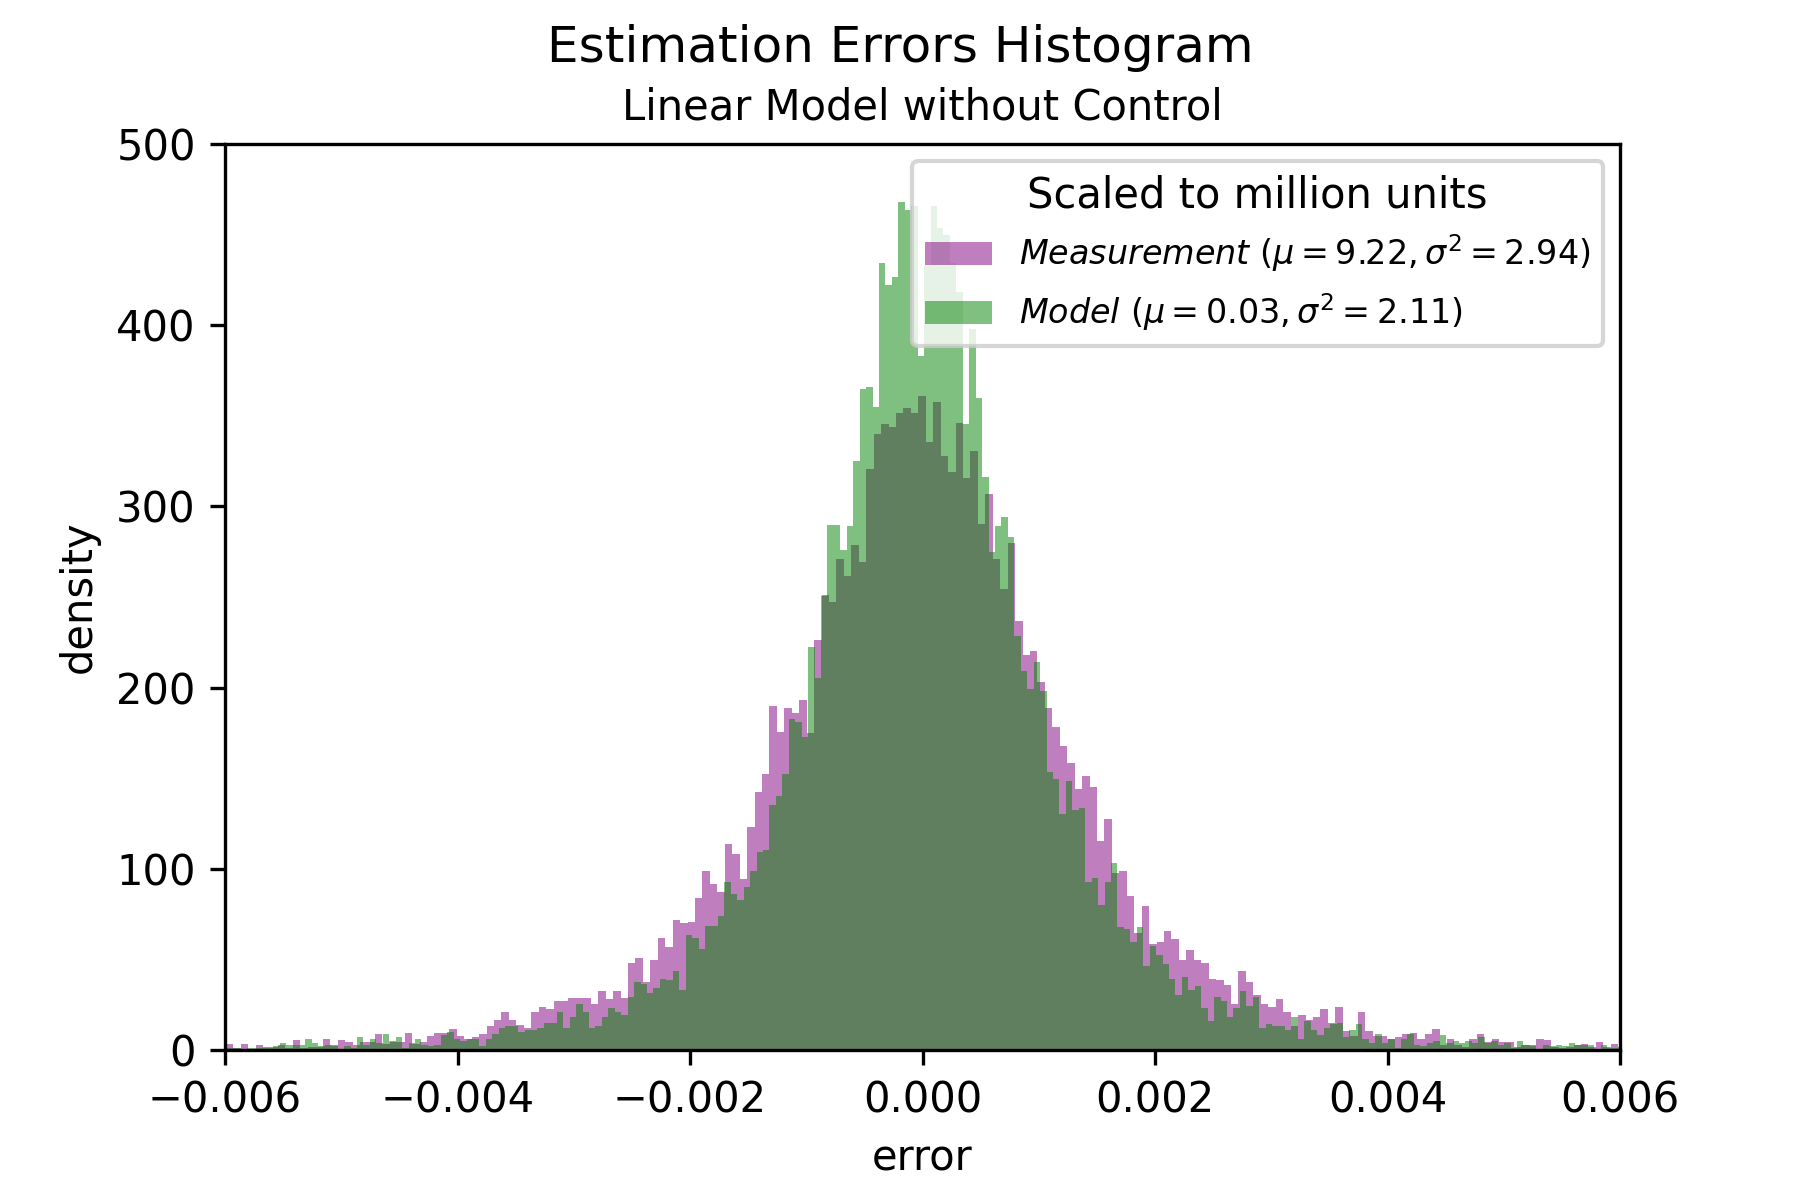
\includegraphics[width=0.5\textwidth]{Errors Histogram [Linear Model without Control].png}
\centering
\end{figure}
\end{مشاهده}

\begin{مشاهده}
همان‌طور که اشاره کردیم، فرض می‌کنیم دینامیک مدل دچار تغییرات سریع نمی‌شود. این نکته در نمودار زیر به صورت طیف‌های پیوسته قابل مشاهده است. هم‌چنین در نمودار زیر این نکته قابل توجه وجود دارد که ضرایب بزرگ‌تر و تاثیرگذارتر در مدل خطی پیشنهاد شده، به لحظات نزدیک‌تر به لحظه حال مرتبط می‌شوند. این نیز مشاهده‌ای است که انتظارش را داشتیم.

\begin{figure}[h]
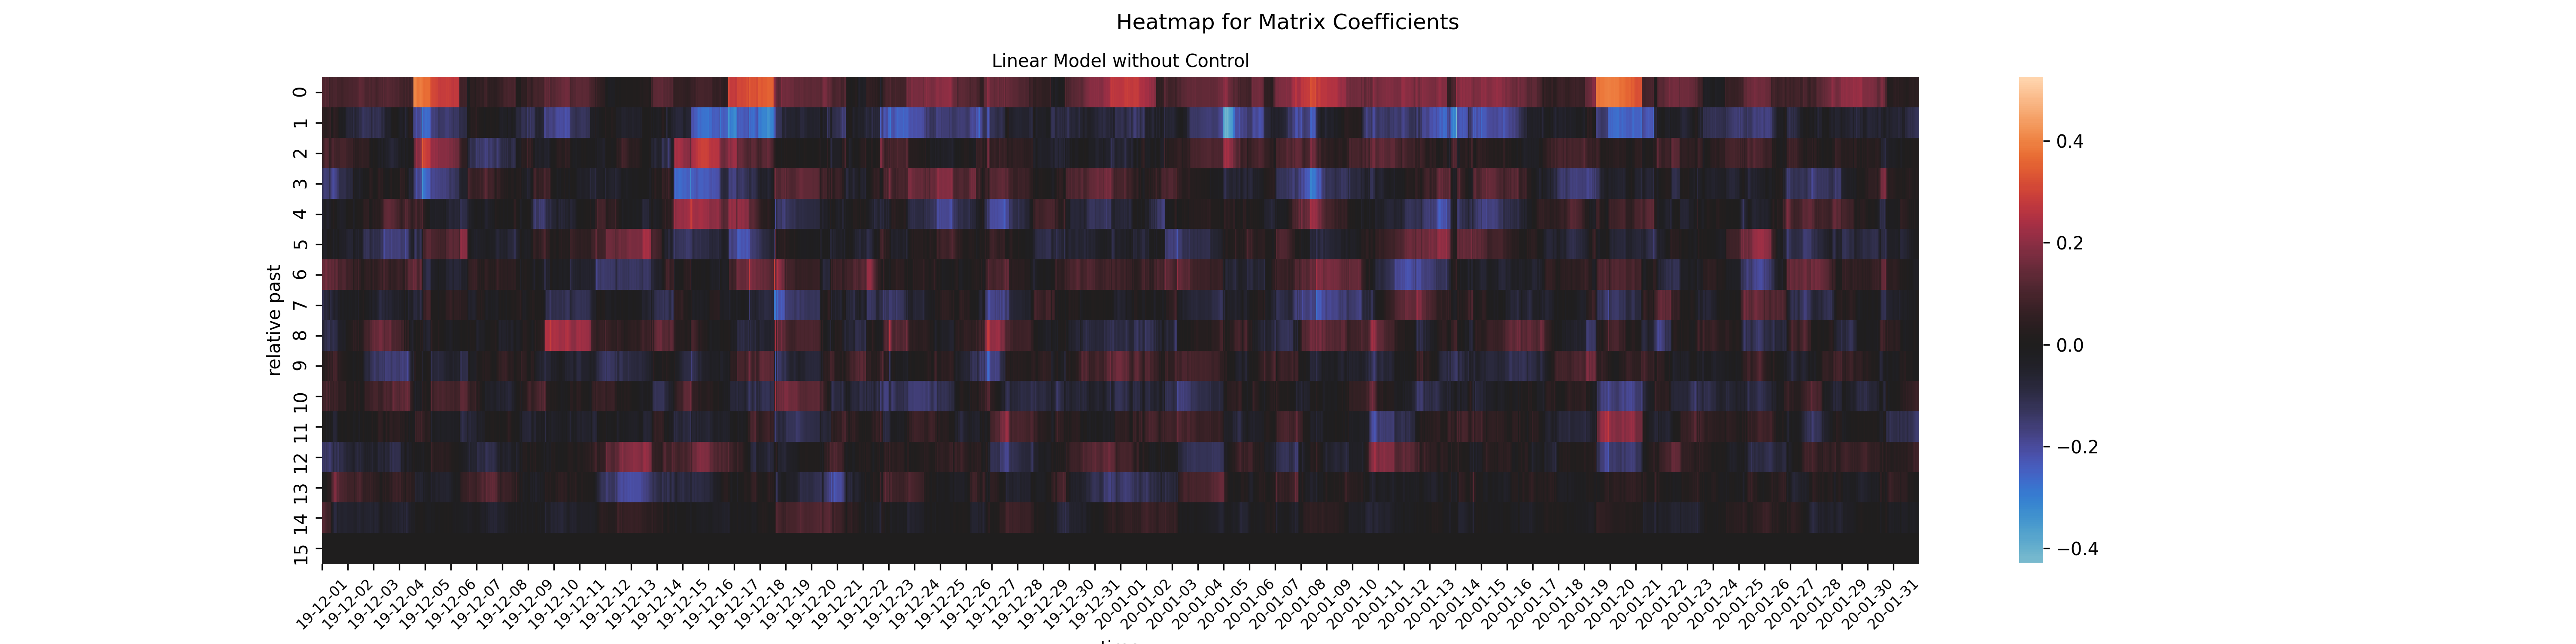
\includegraphics[width=1.1\textwidth]{Heatmap [Linear Model without Control].png}
\centering
\end{figure}
\end{مشاهده}

\begin{نتیجه}
در شکل می‌توان خروجی فیلتر کالمن را بر روی مدل خطی در هر لحظه به ازای یک پنجره خاص زمانی مشاهده کرد.

\begin{figure}[h]
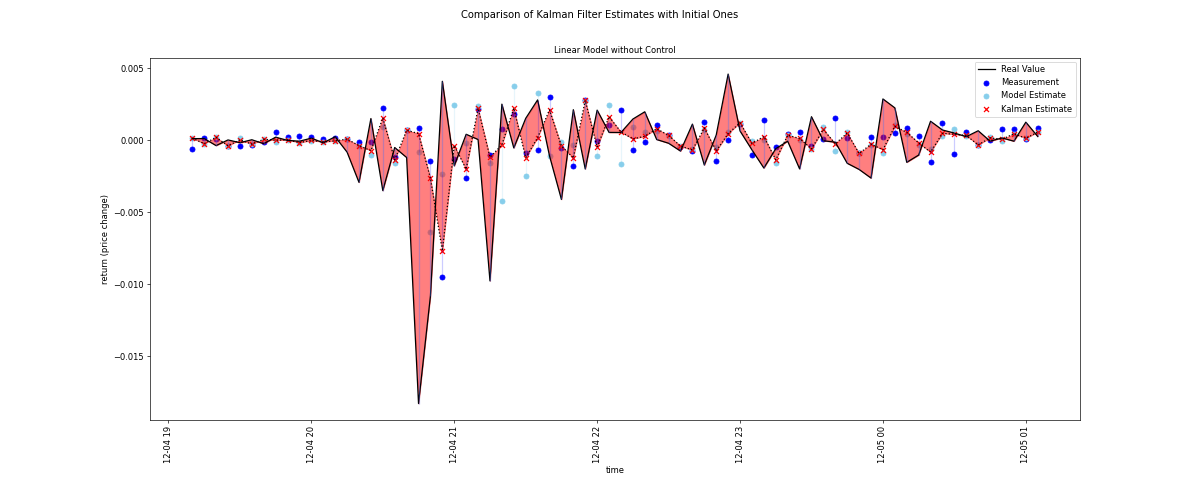
\includegraphics[width=1\textwidth]{Returns and Kalman Filtering [Linear Model without Control].png}
\centering
\end{figure}
\end{نتیجه}

\subsubsection{مدل ۲: دینامیک خطی همراه با کنترل}

\subsubsection{مدل ۳: دینامیک خطی حساس به زمان}

\subsubsection{مدل ۴: دینامیک خطی با ماتریس چگال}



% --------------------------------------------- %
\section{فیلتر کالمن تعمیم‌یافته}
% --------------------------------------------- %

\subsection{تعریف}
\subsection{پیاده‌سازی}
\subsubsection{مدل ۵: دینامیک درجه ۲ بدون کنترل}
\subsubsection{مدل ۶: دینامیک درجه ۲ همراه با کنترل خطی}
\subsubsection{مدل ۷: دینامیک شبکه عصبی}
\subsubsection{مدل ۸: دینامیک مشتق‌ناپذیر}


\section{فیلتر کالمن سریع}


\section{فیلتر کالمن با چند مدل}
\subsection{جمع‌بندی مدل‌های ارایه شده}
\subsection{تعمیم فیلتر کالمن به چند مدل موازی}
\subsubsection{تعمیم ضرایب کالمن}
\subsubsection{ترکیب چند فیلتر}

\section{ارجاع و منابع}



















































\section{گزاره‌های کاربردی}
در این قسمت، مطالب و لم‌هایی را که در حل تمرینات مورد استفاده قرار می‌دهیم، بیان و اثبات می‌کنیم.


\section{تمرینات}
در ادامه همگی تمرینات فصل دوم حل شده‌اند. اما تنها تمرینات
\lr{2.6}
الی
\lr{2.9}
تحویلی بوده‌اند که در کنار آن‌ها یک علامت * زده شده است.

% --------------- Problem 2.6 --------------- %
\bigbreak
\begin{prob}
توالی‌های
\lr{DNA}
$S_1$
و
$S_2$،
به ترتیب با طول‌های
$n$
و
$m$
داده شده‌اند. آیا می‌توانید یک الگوریتم کارا ارائه کنید که تعداد کل هم‌ترازی‌های بین
$S_1$
و
$S_2$
را برگرداند؟ پیچیدگی زمانی این الگوریتم پیشنهادی چیست؟
\end{prob}


\begin{حل}
جدول برنامه‌ریزی پویا برای الگوریتم
\lr{Needleman-Wunsch}
را
$M$
در نظر می‌گیریم. بنا به نحوه ساخت این جدول، می‌دانیم هر هم‌ترازی بین رشته‌های
$S$
و
$T$
یک مسیر از درایه ابتدایی سمت چپ و بالای جدول به درایه انتهایی سمت راست و پایین جدول است که تنها یال‌های مجاز در آن، حرکت به سمت راست یا پایین یا حرکت قطری راست-پایین است. برعکس هر چنین مسیری یک هم‌ترازی را معین می‌کند و لذا مجموعه هم‌ترازی‌ها(ی بدون ستون‌های بدیهی اضافه) با مسیر‌های
$M[0,0]\rightarrow M[n,m]$
در تناظر یک‌به‌یک است. در این بین، ادعا می‌کنیم که مسیر‌های
$P$
که کلیه یال‌های آن‌ها، یعنی مجموعه
$\{v := M[i,j]\rightarrow M[i+b_1,j+b_2] | v\in P, \s b_1, b_2 = 0,1 \}$،
بهینه باشند، تنها مسیرهای بهینه هستند. منظور از یال بهینه
$e = M[i,j]\rightarrow M[i+b_1,j+b_2]$
آن است که
$e$
در جدول برنامه‌ریزی پویا ظاهر شود. یا به عبارت دیگر، درایه
$M[i+b_1,j+b_2]$
بتواند مقدار بهینه خود را با صرف هزینه عملیات نظیر لازم، از درایه
$M[i,j]$
اخذ کند. اثبات این ادعا با برهان خلف کار دشواری نیست. کافیست فرض کنیم یالی از
$P'$
مانند
$e'$
موجود است که در جدول
$M$
نیست و این یال، آخرین یال با خاصیت مذکور باشد. مثلا
$e' = M[i',j']\rightarrow M[i'+b_1,j'+b_2]$.
اکنون به استقرای ریاضی روی مکان این یال، می‌توان به سادگی نشان داد که مقدار درایه
$M[i'+b_1,j'+b_2]$
در جدول، از هزینه هم‌ترازی متناظر با
$P'$
تا انتهای یال
$e'$
اکیدا کمتر است و لذا
$P'$
نمی‌تواند یک هم‌ترازی بهینه باشد.

پس تعداد مسیر‌های جهت‌دار را می‌خواهیم که از
$M[0,0]$
شروع شده و به
$M[n,m]$
ختم می‌شوند. برای شمارش این مسیر‌ها، جدول
$V$
را از ابعاد مساوی با
$M$
می‌سازیم و همه مقادیر آن را در ابتدا برابر با صفر تعیین می‌کنیم. به کمک رابطه بازگشتی زیر و با یک بار پیمایش جدول
$V$،
مقدار خانه
$V[0,0]$
را به عنوان پاسخ باز می‌گردانیم. (در رابطه زیر،
$\delta$
همان تابع دلتای دیراک است و
$M[i,j]\rightarrow M[i',j'] \in M$
یعنی یال فوق، آنطور که تعریف کردیم، بهینه باشد.

$$
\begin{cases}
V[n, m] = 1 \\
V[i,j] = \Sigma_{b_1,b_2 \in \{0,1\}}
V[i+b_1, j+b_2]\delta_{M[i,j]\rightarrow M[i+b_1,j+b_2] \in M}
\end{cases}
$$

اثبات اینکه رابطه بازگشتی فوق، به درستی تعداد مسیر‌های
$M[i,j]$
به
$M[n,m]$
را باز می‌گرداند، سرراست است. در این خصوص توجه می‌کنیم که تعداد مسیرهای با راس شروع
$M[i,j]$
که به
$M[n,m]$
ختم می‌شوند،
طبق اصل جمع برابر است با جمع تعداد مسیرهای از
$M[i+b_1,j+b_2]$
به
$M[n,m]$
که یال
$M[i,j]\rightarrow M[i+b_1,j+b_2]$
موجود باشد.

واضح است که پیچیدگی این الگوریتم، برابر با پیچیدگی الگوریتم
\lr{Needleman-Wunsch}
خواهد بود به علاوه
$O(mn)$
پیچیدگی زمانی برای پیمایش جدول
$V$،
و
$O(mn) + O(\min(m,n)) = O(mn)$
پیچیدگی حافظه برای نگه‌داری جدول
$M$
و آپدیت ستونی یا سطری
$V$.
\end{حل}



% --------------- Problem 2.7 --------------- %
\bigbreak
\begin{prob}
هم‌ترازی زیر را در نظر بگیرید،

\begin{align*}
A \s C \s \dash \s G \s G \s T \s T \s A \s T \s \dash \\
\dash \s C \s T \s G \s G \s \dash \s \dash \s A \s T \s C \\
\end{align*}

به همراه ماتریس امتیاز زیر.

$$
\arraycolsep=1.4pt\def\arraystretch{1.5}
\begin{array}{c|c|c|c|c}
 & A & C & G & T \\ \hline
A & 1 & & & \\ \hline
C & -1 & 2 & & \\ \hline
G & -1 & -2 & 1 & \\ \hline
T & -2 & -1 & -2 & 1
\end{array}
$$

\begin{enumerate}
\item{
فرض کنید برای یک گپ از سایز
$g$
پنالتی
$-5-g$
را در نظر بگیریم. امتیاز هم‌ترازی فوق را بر اساس این پنالتی و ماتریس امتیاز داده شده بیابید.


\begin{حل}
چهار گپ داریم که به ترتیب در مکان‌های
$i = [1], [3], [6, 7], [10]$
هستند. لذا پنالتی یا همان امتیاز منفی تحمیلی این گپ‌ها به ترتیب برابر با
$-6, -6, -7, -6$
خواهد بود. امتیاز سایر بخش‌های هم‌ترازی از روی ماتریس امتیاز قابل محاسبه خواهد بود و مجموع امتیاز برابر است با،

\begin{align*}
-6 + 2 - 6 + 1 + 1 - 7 + 1 + 1 - 6
\end{align*}

یا
$-19$.
\end{حل}


}
\item{
آیا هم‌ترازی فوق بهینه است؟ اگر پاسخ منفیست، امتیاز هم‌ترازی بهینه و یک هم‌ترازی نظیر با آن را ارائه دهید.


\begin{حل}
خیر. هم‌ترازی‌های زیر امتیازی برابر با
$-8$
دارند و نتیجتا هم‌ترازی سوال بهینه نیست.

\begin{align*}
A \s C \s G \s G \s T \s T \s A \s T \qquad \qquad & A \s C \s G \s G \s T \s T \s A \s T \\
C \s T \s G \s G \s A \s T \s C \s \dash \qquad \qquad & C \s T \s G \s G \s A \s T \s \dash \s C \\
\end{align*}

اکنون به کمک رابطه بازگشتی زیر ثابت می‌کنیم هم‌ترازی‌های ارائه شده بهینه هستند (که در آن رابطه
$A\rightarrow B$
به این معنی است که خانه
$B$
جدول، مقدار بهینه خود را از خانه
$A$
دریافت کرده است).

$$
M[i+1, j+1] = \max
\begin{cases}
M[i+1,j] - 6 & \quad M[i+1,j-1] \not\rightarrow M[i+1,j] \\
M[i+1,j] - 1 & \quad M[i+1,j-1] \rightarrow M[i+1,j] \\
M[i,j+1] - 6 & \quad M[i-1,j+1] \not\rightarrow M[i,j+1] \\
M[i,j+1] - 1 & \quad M[i-1,j+1] \rightarrow M[i,j+1] \\
M[i,j] + w(S[i+1],T[j+1]) \\
\end{cases} 
$$

جدول بهترین هم‌ترازی توالی‌های
$S[1,\dots,i]$
و
$T[1,\dots,j]$
در ادامه آمده است:

$$
\arraycolsep=1.4pt\def\arraystretch{1.5}
\begin{array}{c|cccccccccccccccccc} 
 & \dash & & A & & C & & G & & G & & T & & T & & A & & T \\
 
\hline
\dash & \circled{0} & \ra & -6 &\ra & -7 &\ra & -8 &\ra & -9 &\ra & -10 &\ra & -11 &\ra & -12 &\ra & -13 \\

 &\da &\sea & &\sea & &\sea & &\sea & &\sea & &\sea & &\sea & &\sea & \\
 
C & -6 & & \circled{-1} & & -4 & & -9 & & -10 & & -10 & & -11 & & -12 & & -13 \\

 &\da & &\da &\sea & &\sea & &\sea & &\sea & &\sea & &\sea & &\sea & \\
 
T & -7 & & -7 & & \circled{-2} & & -6 & & -11 & & -9 & & -9 & & -13 & & -11 \\

 &\da &\sea &\da & &\da &\sea & &\sea & & & &\sea & &\sea & &\sea & \\
 
G & -8 & & -8 & & -8 & & \circled{-1} & & -5 &\ra & -11 & & -11 & & -10 & & -15 \\

 & \da &\sea & \da & & \da &\sea &\da &\sea & & & & & & & & & \\
 
G & -9 & & -9 & & -9 & & -7 & & \circled{0} &\ra & -6 &\ra & -7 &\ra & -8 &\ra & -9 \\

 & \da &\sea & &\sea & \da & &\da & &\da &\sea & &\sea & &\sea & &\sea & \\
 
A & -10 & & -8 & & -10 & & -8 & & -6 & & \circled{-2} & \ra & -8 & & -6 & & -10 \\

 &\da &\sea & &\sea & & &\da & &\da &\sea & &\sea & & & &\sea & \\
 
T & -11 & & -12 & & -9 & & -9 & & -7 & & -5 & & \circled{-1} &\ra & \circled{-7} & & -5 \\

 & \da &\sea & &\sea & & &\da & &\da &\sea & &\sea & &\sea & &\sea & \\
 
C & -12 & & -12 & & -10 & & -10 & & -8 & & -8 & & -6 & & \circled{-2} & \ra & \circled{-8} 
\end{array}
$$

می‌توان از روی جدول مشاهده کرد که تنها همین دو هم‌ترازی بهینه متمایز را داریم.
\end{حل}


}
\item{
یک ماتریس امتیاز و یک تابع پنالتی گپ ارائه کنید به قسمی که هم‌ترازی داده شده در بالا، یک هم‌ترازی بهینه شود.


\begin{حل}
ادعا می‌کنیم ماتریس امتیاز زیر به همراه پنالتی ساده
$-g$
برای گپ از سایز
$g$،
هم‌ترازی مورد نظر را یک هم‌ترازی بهینه می‌شناسد.

$$
\arraycolsep=1.4pt\def\arraystretch{1.5}
\begin{array}{c|c|c|c|c}
 & A & C & G & T \\ \hline
A & 10 & & & \\ \hline
C & -1 & 1 & & \\ \hline
G & -1 & -1 & 100 & \\ \hline
T & -1 & -1 & -1 & 1
\end{array}
$$

با توجه به امتیاز هم‌خوانی
$G$
واضح است که هر هم‌ترازی بهینه برای این ماتریس امتیاز، باید حتما
$G$ها
را مقابل هم قرار دهد. اکنون برای قسمت‌های
$S[1,2]$
و
$T[1,2]$
نیز واضح است که قرار دادن
$C$های
این دو زیررشته در مقابل هم، امتیاز هم‌ترازی را افزایش می‌دهد. برای زیررشته‌های طرف دیگر
$S[4,\dots,8]$
و
$T[4,\dots,7]$
نیز با توجه به امتیاز هم‌خوانی
$A$
می‌دانیم حتما باید تک عنصر
$A$
موجود در این دو زیررشته هم‌خوان باشد و لذا نشان دادیم هم‌ترازی داده شده یک هم‌ترازی بهینه برای ماتریس امتیاز و پنالتی مفروض ماست.
\end{حل}


}
\end{enumerate}
\end{prob}



% --------------- Problem 2.8 --------------- %
\bigbreak
\begin{prob}
الگوی
$P$
از طول
$m$
و رشته
$T$
از طول
$n$
داده شده‌اند. فرض کنید
$P^n$
توالی از طول
$mn$
باشد که از کنار هم قرار دادن
$n$
کپی از
$P$
ساخته شده است. هم‌چنین فرض کنید امتیاز هم‌خوانی برابر با
$1$
و امتیاز ناهم‌خوانی، حذف، و اضافه برابر با
$-1$
باشد. آیا می‌توانید الگوریتمی با پیچیدگی زمانی
$O(nm)$
ارائه کنید که قادر به محاسبه هم‌ترازی موضعی بهینه بین
$P^n$
و
$T$
باشد؟
\end{prob}


\begin{حل}
فرض کنیم جدول برنامه‌ریزی پویای هم‌ترازی موضعی رشته‌های
$P$
و
$T$
را داریم و آن را
$M$
بنامیم (موقتا فرض کنیم سطر و ستون
$\dash$
در
$M$
ظاهر نشده باشند.). توجه‌ می‌کنیم که اگر گراف جهت‌دار مربوط به این جدول را
$n$
مرتبه کپی کنیم و کنار هم بگذاریم، و یال‌های جهت‌دار بین درایه‌های ستون آخر جدول
$M$
و ستون اول جدول
$M$
بعدی را نیز محاسبه و ترسیم کنیم، گراف جهت‌دار متناظر با جدول برنامه‌ریزی پویای مساله بهترین هم‌ترازی موضعی
$P^n$
و
$T$
حاصل می‌شود. توجه می‌کنیم که هر هم‌ترازی موضعی معادل با مسیری در این گراف جهت‌دار است. اما به دلیل ساختار این گراف جهت‌دار، می‌توانیم به جای بررسی آن، یال‌های مربوط به ستون آخر جدول
$M$
را مستقیما به ستون اول
$M$
وصل کنیم و به دنبال یک مسیر مناسب در گراف جهت‌دار حاصل
$D$
 بگردیم. در واقع به کمک آنچه در مسایل قبل بیان و ثابت کردیم، می‌توانیم فرض کنیم هر هم‌ترازی بهینه موضعی توالی‌های
$P^n$
و
$T$
معادل با یک مسیر در گراف
$D$
است.

یال‌های
$D$
را بر اساس اینکه یک هم‌خوانی را بیان می‌کنند یا خیر، به ترتیب به دو رنگ آبی و قرمز رنگ‌آمیزی کنیم. امتیازی که هر یال آبی به هم‌ترازی موضعی متناظر با مسیر‌های شامل خودش اضافه می‌کند،
$+1$
خواهد بود و امتیاز هر یال قرمز
$-1$.
پس در گراف
$D$
به دنبال مسیری هستیم که تفاضل تعداد یال‌های آبی از قرمزش بیشینه باشد. به عنوان یک نکته توجه می‌کنیم که طول
$P^n$
از طول
$T$
کمتر نیست و لذا هر مسیر در
$D$،
چون حداکثر
$n-1$
بار به سمت پایین یال دارد، حداکثر
$n-1$
بار ستون آخر
$M$
را رد می‌کند و لذا هم‌ترازی معادلی در
$P^n$
دارد.

برای مثال به جدول‌ زیر که برای توالی‌های
$P:=TTC$
و
$T:=AGTT$
ترسیم شده است، (پیکان‌های خاکستری مربوط به جدول هم‌ترازی سراسری هستند. پیکان‌های قرمز و آبی، مطلوب ماست.)

$$
\arraycolsep=1.4pt\def\arraystretch{1.5}
\begin{array}{c|ccccccc} 

 & \dash & & T & & T & & G \\
\hline

\dash & \circled{0} & \ra & \circled{0} & \ra & \circled{0} & \ra & \circled{0} \\

 & \da & \sea & & \sea & & \sea & \\

A & \circled{0} & & \circled{0} & \ra & \circled{0} & \ra & \circled{0} \\

 & \da & \sea & \da & \sea & & \bluesea &  \\

G & \circled{0} & & \circled{0} & & \circled{0} & & \circled{1} \\

 & \da & \bluesea & & \bluesea & & & \redda \\

T & \circled{0} & & \circled{1} & & \circled{1} & \redra & \circled{0} \\

 & \da & \bluesea & \da & \bluesea & & & \\

T & \circled{0} & & \circled{1} & & \circled{2} & \redra & \circled{1}

\end{array}
$$

و جدول زیر که مربوط به توالی‌های
$P^4 = TTGTTGTTGTTG$
و
$T = AGTT$
است، توجه می‌کنیم.

$$
\arraycolsep=1.4pt\def\arraystretch{1.5}
\begin{array}{c|ccccccc;{2pt/2pt}c;{2pt/2pt}ccccc;{2pt/2pt}c;{2pt/2pt}ccccc;{2pt/2pt}c;{2pt/2pt}ccccc} 

 & \dash & & T & & T & & G & & T & & T & & G & & T & & T & & G & & T & & T & & G \\
\hline

\dash & \circled{0} & \ra & \circled{0} & \ra & \circled{0} & \ra & \circled{0} & \ra & \circled{0} & \ra & \circled{0} & \ra & \circled{0} & \ra & \circled{0} & \ra & \circled{0} & \ra & \circled{0} & \ra & \circled{0} & \ra & \circled{0} & \ra & \circled{0}\\

 & \da & \sea & & \sea & & \sea & & \sea & & \sea & & \sea & & \sea & & \sea & & \sea & & \sea & & \sea & & \sea & \\

A & \circled{0} & & \circled{0} & \ra & \circled{0} & \ra & \circled{0} & \ra & \circled{0} & \ra & \circled{0} & \ra & \circled{0} & \ra & \circled{0} & \ra & \circled{0} & \ra & \circled{0} & \ra & \circled{0} & \ra & \circled{0} & \ra & \circled{0} \\

 & \da & \sea & \da & \sea & & \bluesea & & & \da & \sea & & \bluesea & & & \da & \sea & & \bluesea & & & \da & \sea & & \bluesea & \\

G & \circled{0} & & \circled{0} & & \circled{0} & & \circled{1} & \redra & \circled{0} & & \circled{0} & & \circled{1} & \redra & \circled{0} & & \circled{0} & & \circled{1} & \redra & \circled{0} & & \circled{0} & & \circled{1} \\

 & \da & \bluesea & & \bluesea & & & \redda & \bluesea & & \bluesea & & & \redda & \bluesea & & \bluesea & & & \redda & \bluesea & & \bluesea & & & \redda \\

T & \circled{0} & & \circled{1} & & \circled{1} & \redra & \circled{0} & & \circled{2} & & \circled{1} & \redra & \circled{0} & & \circled{2} & & \circled{1} & \redra & \circled{0} & & \circled{2} & & \circled{1} & \redra & \circled{0} \\

 & \da & \bluesea & \da & \bluesea & & & & \bluesea & \redda & \bluesea & & & & \bluesea & \redda & \bluesea & & & & \bluesea & \redda & \bluesea & & & \\

T & \circled{0} & & \circled{1} & & \circled{2} & \redra & \circled{1} & & \circled{1} & & \circled{3} & \redra & \circled{2} & & \circled{1} & & \circled{3} & \redra & \circled{2} & & \circled{1} & & \circled{3} & \redra & \circled{2}

\end{array}
$$

اکنون الگوریتیمی ارائه می‌کنیم که در زمان
$O(mn)$
بتواند بهترین امتیاز در بین همه مسیر‌های شروع شونده از هر درایه
$M[i,j]$
را به صورت پویا محاسبه کند. ماتریس امتیازات
$V$
را هم‌ابعاد با
$M$
در نظر میگیریم و مقادیر اولیه درایه‌هایش را برابر با ۰ قرار می‌دهیم و سپس سطرهای
$M$
را از پایین به بالا پیمایش می‌کنیم. برای سطر
$n$ام
قرار می‌دهیم
$V[n,j] = 0$.
(چون هم‌ترازی‌های موضعی را بررسی می‌کنیم، مقادیر منفی با ۰ جایگزین می‌شوند.) می‌توانیم فرض کنیم
$V[i,j]$
بیانگر امتیاز هم‌ترازی بهینه موضعی توالی‌های
$P^n[j+1,\dots,mn]$
و
$T[i+1,\dots,n]$
است (واضح است که هر هم‌ترازی بهینه موضعی را می‌توان فرض کرد از
$P$
یا در واقع از اندیسی بین
1
و
$m$
شروع می‌شود). برای سطرهای بالاتر
$V$
الگوریتم زیر را داریم:

\begin{algorithmic}[1]
\For $i \gets n-1,\ \dots,\ 0$
\For $j \gets 0,\ \dots,\ m$
\State $V[i,j] \gets 0$
\If{$ v_{i,j}\rightarrow v_{i+1,j} \in D $}
\State $V[i,j] \gets \max \{V[i+1,j] - 1,\ V[i,j]\}$
\EndIf
\If{$ v_{i,j}\rightarrow v_{i+1,j+1} \in D$ و یال قرمز باشد}
\State $V[i,j] \gets \max \{V[i+1,j+1] - 1,\ V[i,j]\}$
\EndIf
\If{$ v_{i,j}\rightarrow v_{i+1,j+1} \in D$ و یال آبی باشد}
\State $V[i,j] \gets \max \{V[i+1,j+1] + 1,\ V[i,j]\}$
\EndIf
\EndFor
\State $j_0 \gets \arg \max _j \{ V[i,j] \}$
\For $k \gets 0,\ \dots,\ m$
\State $j \gets j_k \mod (m+1)$
\State $j_+ \gets j_k + 1 \mod (m+1)$
\If{$V[i,j]\rightarrow V[i,j_+] \in D$}
\State $V[i,j_+] \gets \max \{ V[i,j]-1, V[i,j_+] \}$
\EndIf
\EndFor
\EndFor
\end{algorithmic}

واضح است که الگوریتم بالا از مرتبه
$O(mn)$
است و همینطور برای یافتن
$D$
به
$O(mn)$
زمان احتیاج داریم. پس در مجموع به زمان و حافظه
$O(mn)$
نیاز خواهد بود. خطوط ۱۰ تا ۱۵ الگوریتم ارائه شده فوق، در واقع سعی دارند از اطلاعات یال‌های افقی در
$D$
استفاده کنند و از آنجا که این یال‌ها همگی قرمز هستند، درایه ماکسیمم در یک سطر، هیچگاه مقدارش تغییری نمی‌کند. پس با شروع از چنین درایه‌ای می‌توان با یک گردش
$O(m)$
کل مقادیر سطر را آپدیت کرد.
\end{حل}



% --------------- Problem 2.9 --------------- %
\bigbreak
\begin{prob}
دو توالی
\lr{DNA}
$S_1$
و
$S_2$،
به ترتیب با طول‌های
$n$
و
$m$
داده شده‌اند. قصد داریم کم‌ترین تعداد عملیات لازم برای تبدیل
$S_1$
به
$S_2$
را محاسبه کنیم، وقتی عملیات مجاز شامل
$(1)$
اضافه کردن یک عنصر،
$(2)$
حذف یک عنصر،
$(3)$
جایگزینی یک عنصر، و
$(4)$
برعکس کردن یک زیر رشته از
\lr{DNA}
باشد. به علاوه، در مورد عملیات
$(4)$
فرض می‌کنیم که هر گاه بر روی یک بخش از
\lr{DNA}
اعمال شود، عناصر آن بخش دیگر امکان تبدیل شدن به چیز دیگری تحت هیچ یک از چهار عملیات ذکر شده را نخواهند داشت. آیا می‌توانید یک الگوریتم کارا ارائه کنید که کمترین تعداد عملیات لازم برای تبدیل
$S_1$
به
$S_2$
را باز گرداند؟ پیچیدگی زمانی این الگوریتم چه خواهد بود؟
\end{prob}


\begin{حل}
ماتریس
$I$
را در نظر می‌گیریم که در آن،
$I[i_1,i_2;j_1,j_2]$
امتیاز بهینه هم‌ترازی توالی‌های
$S_1[i_1,\dots,i_2]^R$
و
$S_2[j_1,\dots,j_2]$
را تنها با عملیات
(۱)، (۲) و (۳)
نشان می‌دهد. رابطه بازگشتی زیر را برای محاسبه
$I$
در
$O(m^2n^2)$
داریم.

$$
\begin{cases}
I[i+1,i;j_1,j_2] = (j_2-j_1+1)w_{indel} \\
I[i_1, i_2; j+1,j] = (i_2-i_1+1)w_{indel} \\
{I[i_1,i_2;j_1,j_2] = \max
\begin{cases}
I[i_1+1,i_2;j_1,j_2-1] + w(S_1[i_1],S_2[j_2]) \\
I[i_1+1,i_2;j_1,j_2] + w_{indel} \\
I[i_1,i_2;j_1,j_2-1] + w_{indel}
\end{cases}
}
\end{cases}
$$

حال
$D[i,j]$
را برابر با امتیاز هم‌ترازی بهینه بین رشته‌های
$S_1[1\dots i]$
و
$S_2[1\dots j]$
تعریف کنیم (که در آنها هر چهار عملیات مجاز است). توجه می‌کنیم که شرط ثابت ماندن هر زیررشته بعد از اعمال عملیات (۴) معادل با این است که پس از برعکس کردن یک زیررشته، دیگر فقط امکان اعمال مجدد عملیات (۴) برای عناصر این زیررشته وجود ندارد. به عبارت دیگر، می‌توانیم ابتدا عملیات‌های
(۱)، (۲) و (۳) را انجام دهیم. سپس به سراغ عملیات (۴) برویم.

اگر فرض کنیم آخرین مکان اعمال عملیات (۴) در جفت زیررشته
$S_1[1\dots i]$
و
$S_2[1\dots j]$، 
مکان
$(i',j')$
باشد، رابطه بازگشتی زیر را خواهیم داشت:

$$
\begin{cases}
D[0,j] = j \times w_{indel}\\
D[i,0] = i \times w_{indel}\\
D[i,j] = \max
\begin{cases}
D[i-1,j-1] + w(S_1[i],S_2[j])\\
D[i-1,j]+ w_{indel}\\
D[i,j-1] + w_{indel}\\
\max _{1\leq i' \leq i+1,\ 1\leq j' \leq j+1} \{ D[i'-1,j'-1] + I[i',i;j',j] \} - w_{reverse}
\end{cases}
\end{cases}
$$

پیچیدگی زمانی و حافظه برنامه‌ریزی پویای با ضابطه بالا،
$O(m^2n^2)$
است.
\end{حل}



\section{ارجاع و منابع}
\Latincite{Sung}


\bibliographystyle{alpha-persian}
\bibliography{main}


\end{document}